\section{Data}
The following will include an overview and visualisation of the data acquired for the research, and how it was processed.

\subsection{\ac{ehm} Data}
The research was carried out using \ac{ehm} data. This data was recorded by sensors in 231 BR725 engines during a total of \numprint{14045} flights, and returned on a voluntary basis to Rolls-Royce by customers for analysis. Each aircraft using the BR725 has two engines; to minimise the amount of data used, the values used in this thesis were taken from the left engine only.

\begin{figure}
    \centering
    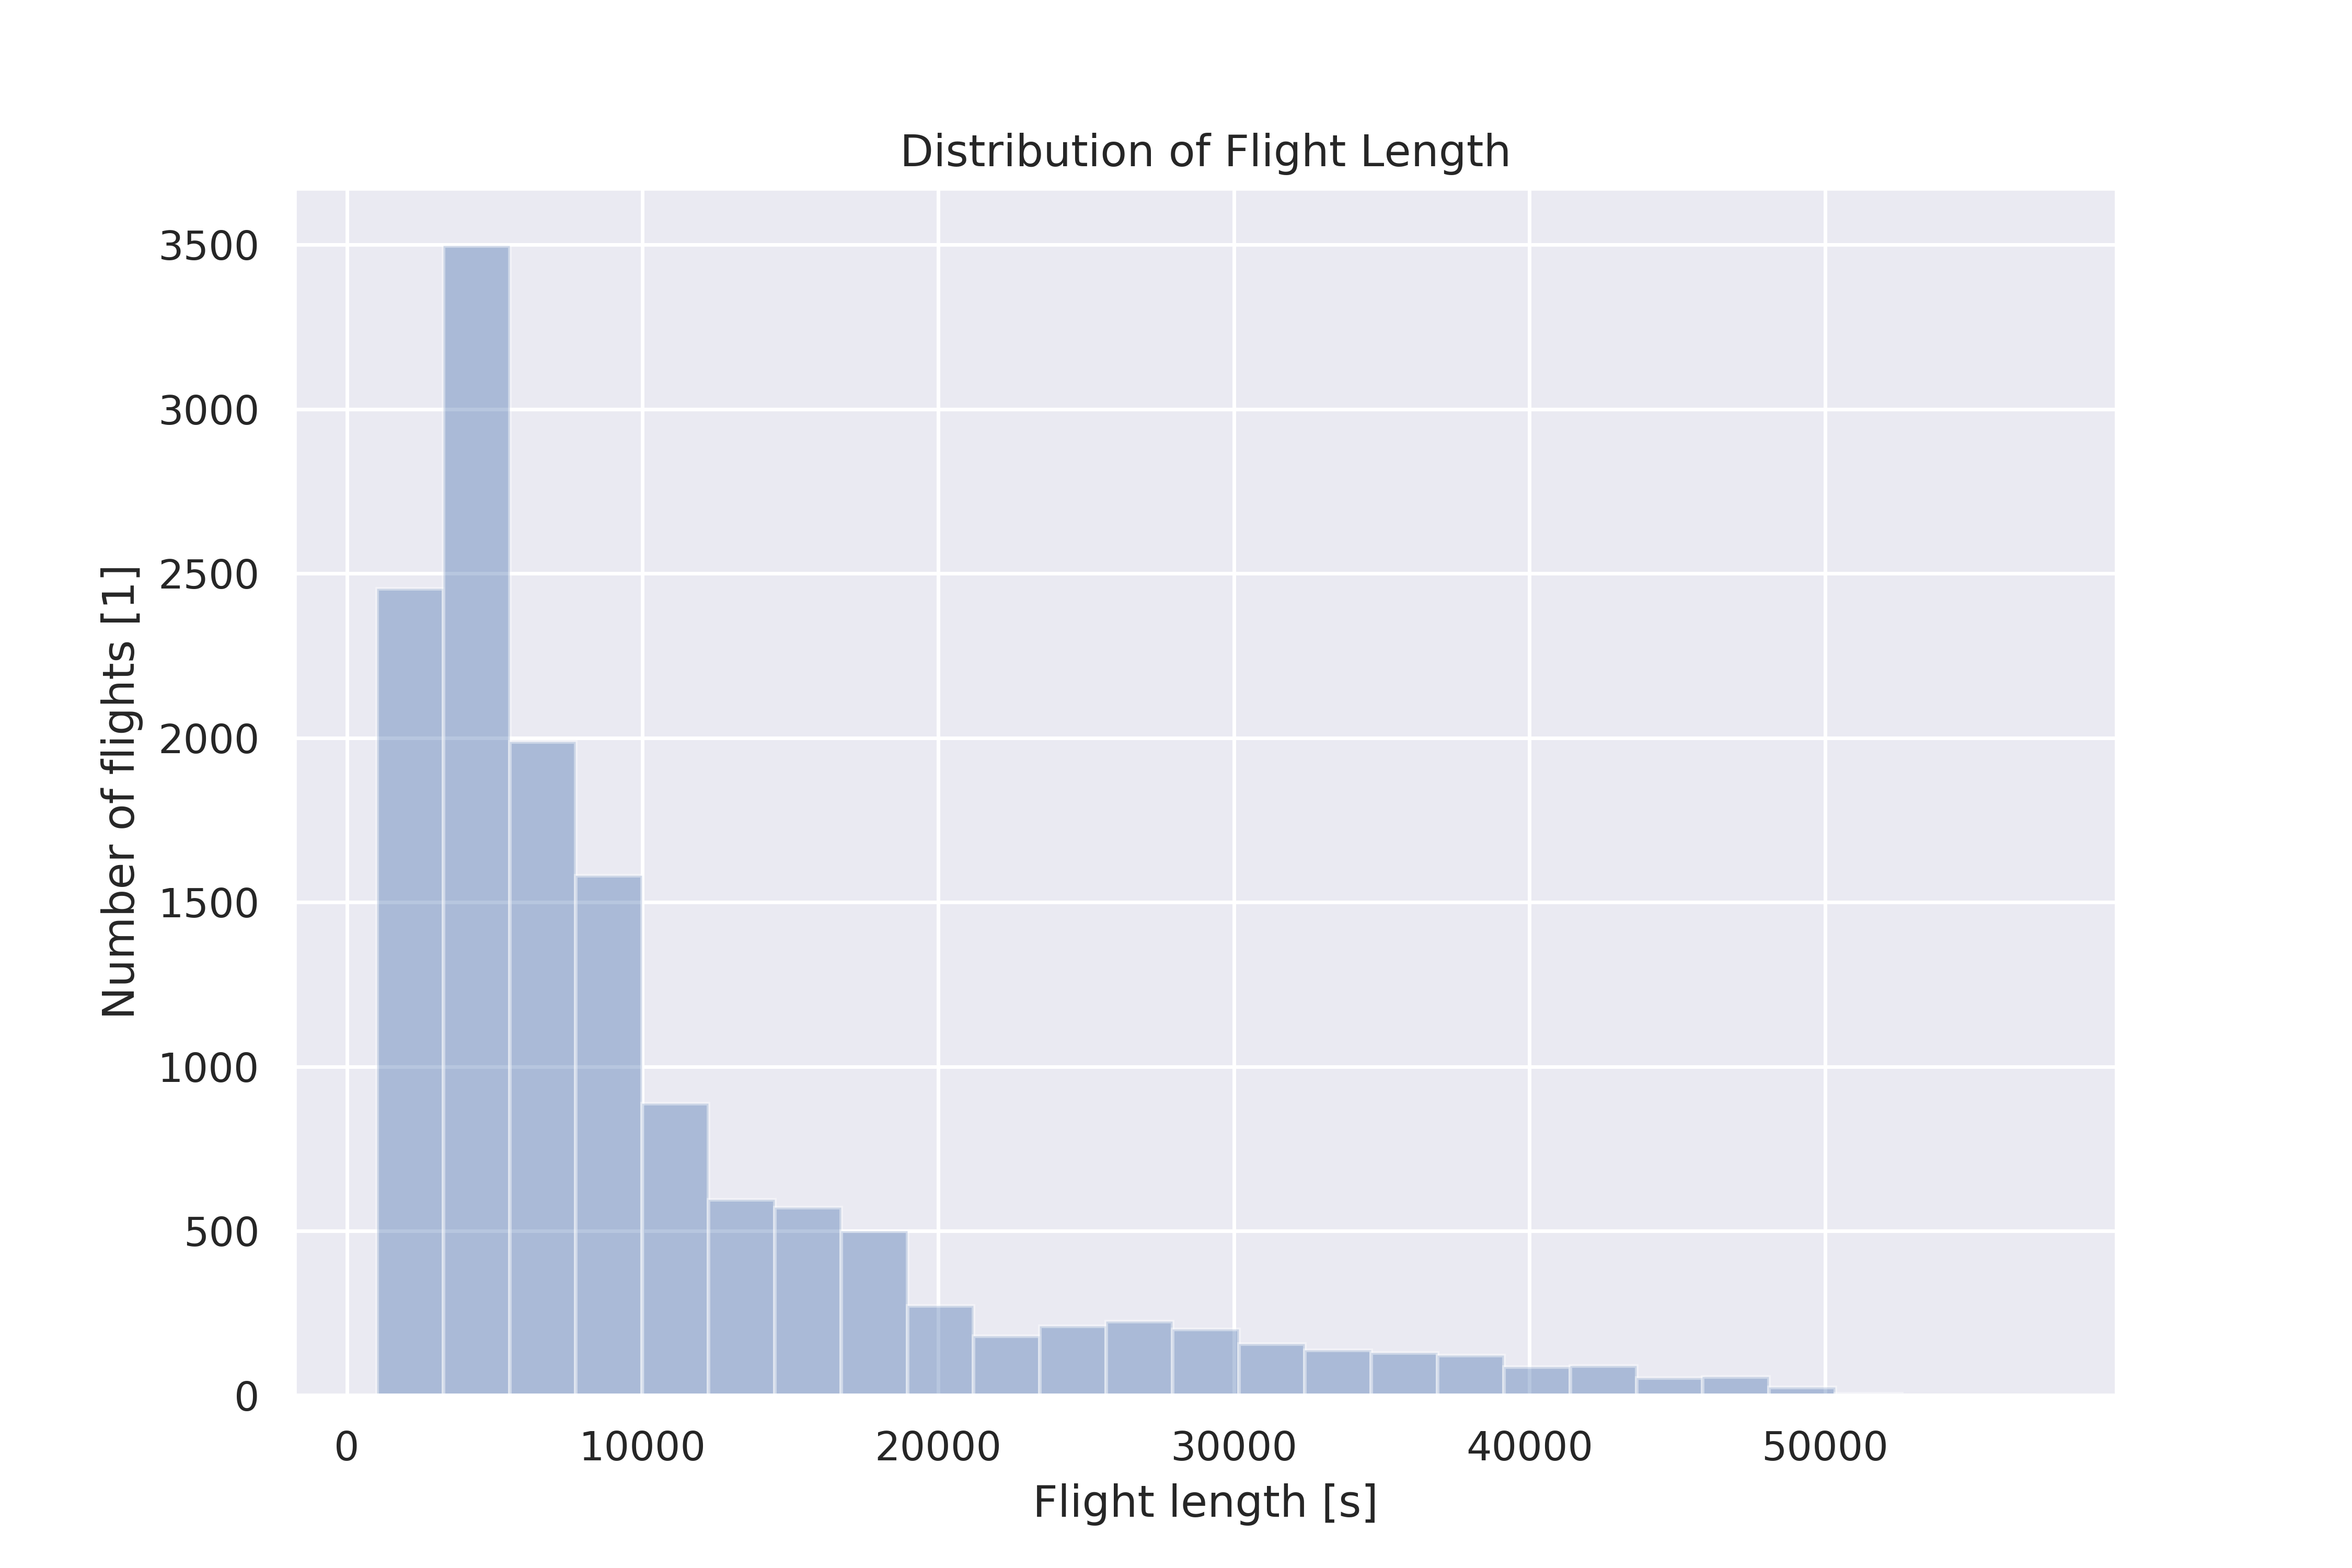
\includegraphics[width=0.9\textwidth]{length_hist}
    \caption{\label{fig:flt_len} A histogram of the lengths of 14045 flights}
\end{figure}

\subsection{Overview}
The flights range in length from \numprint{1013} to \numprint{57062} seconds (approximately 0.28 to 15.85 hours), with a mean length of \numprint{10182.82} seconds and a standard deviation of \numprint{9561.03} seconds (see Figure \ref{fig:flt_len}).

Each flight is summarised in a \ac{csv} file with 216 columns, comprising one timestamp and 215 values per second of recording time.

The four flight parameters extracted were altitude (ALT), rotational speed of the high-pressure shaft (NH), and pressure and temperature of air exiting the compressor (P30 and T30, respectively). These are shown for one randomly selected flight in Figure \ref{fig:flt_example}, with dashed vertical lines representing the boundaries of flight phases (\ref{sec:phases}).

\begin{figure}
    \centering
    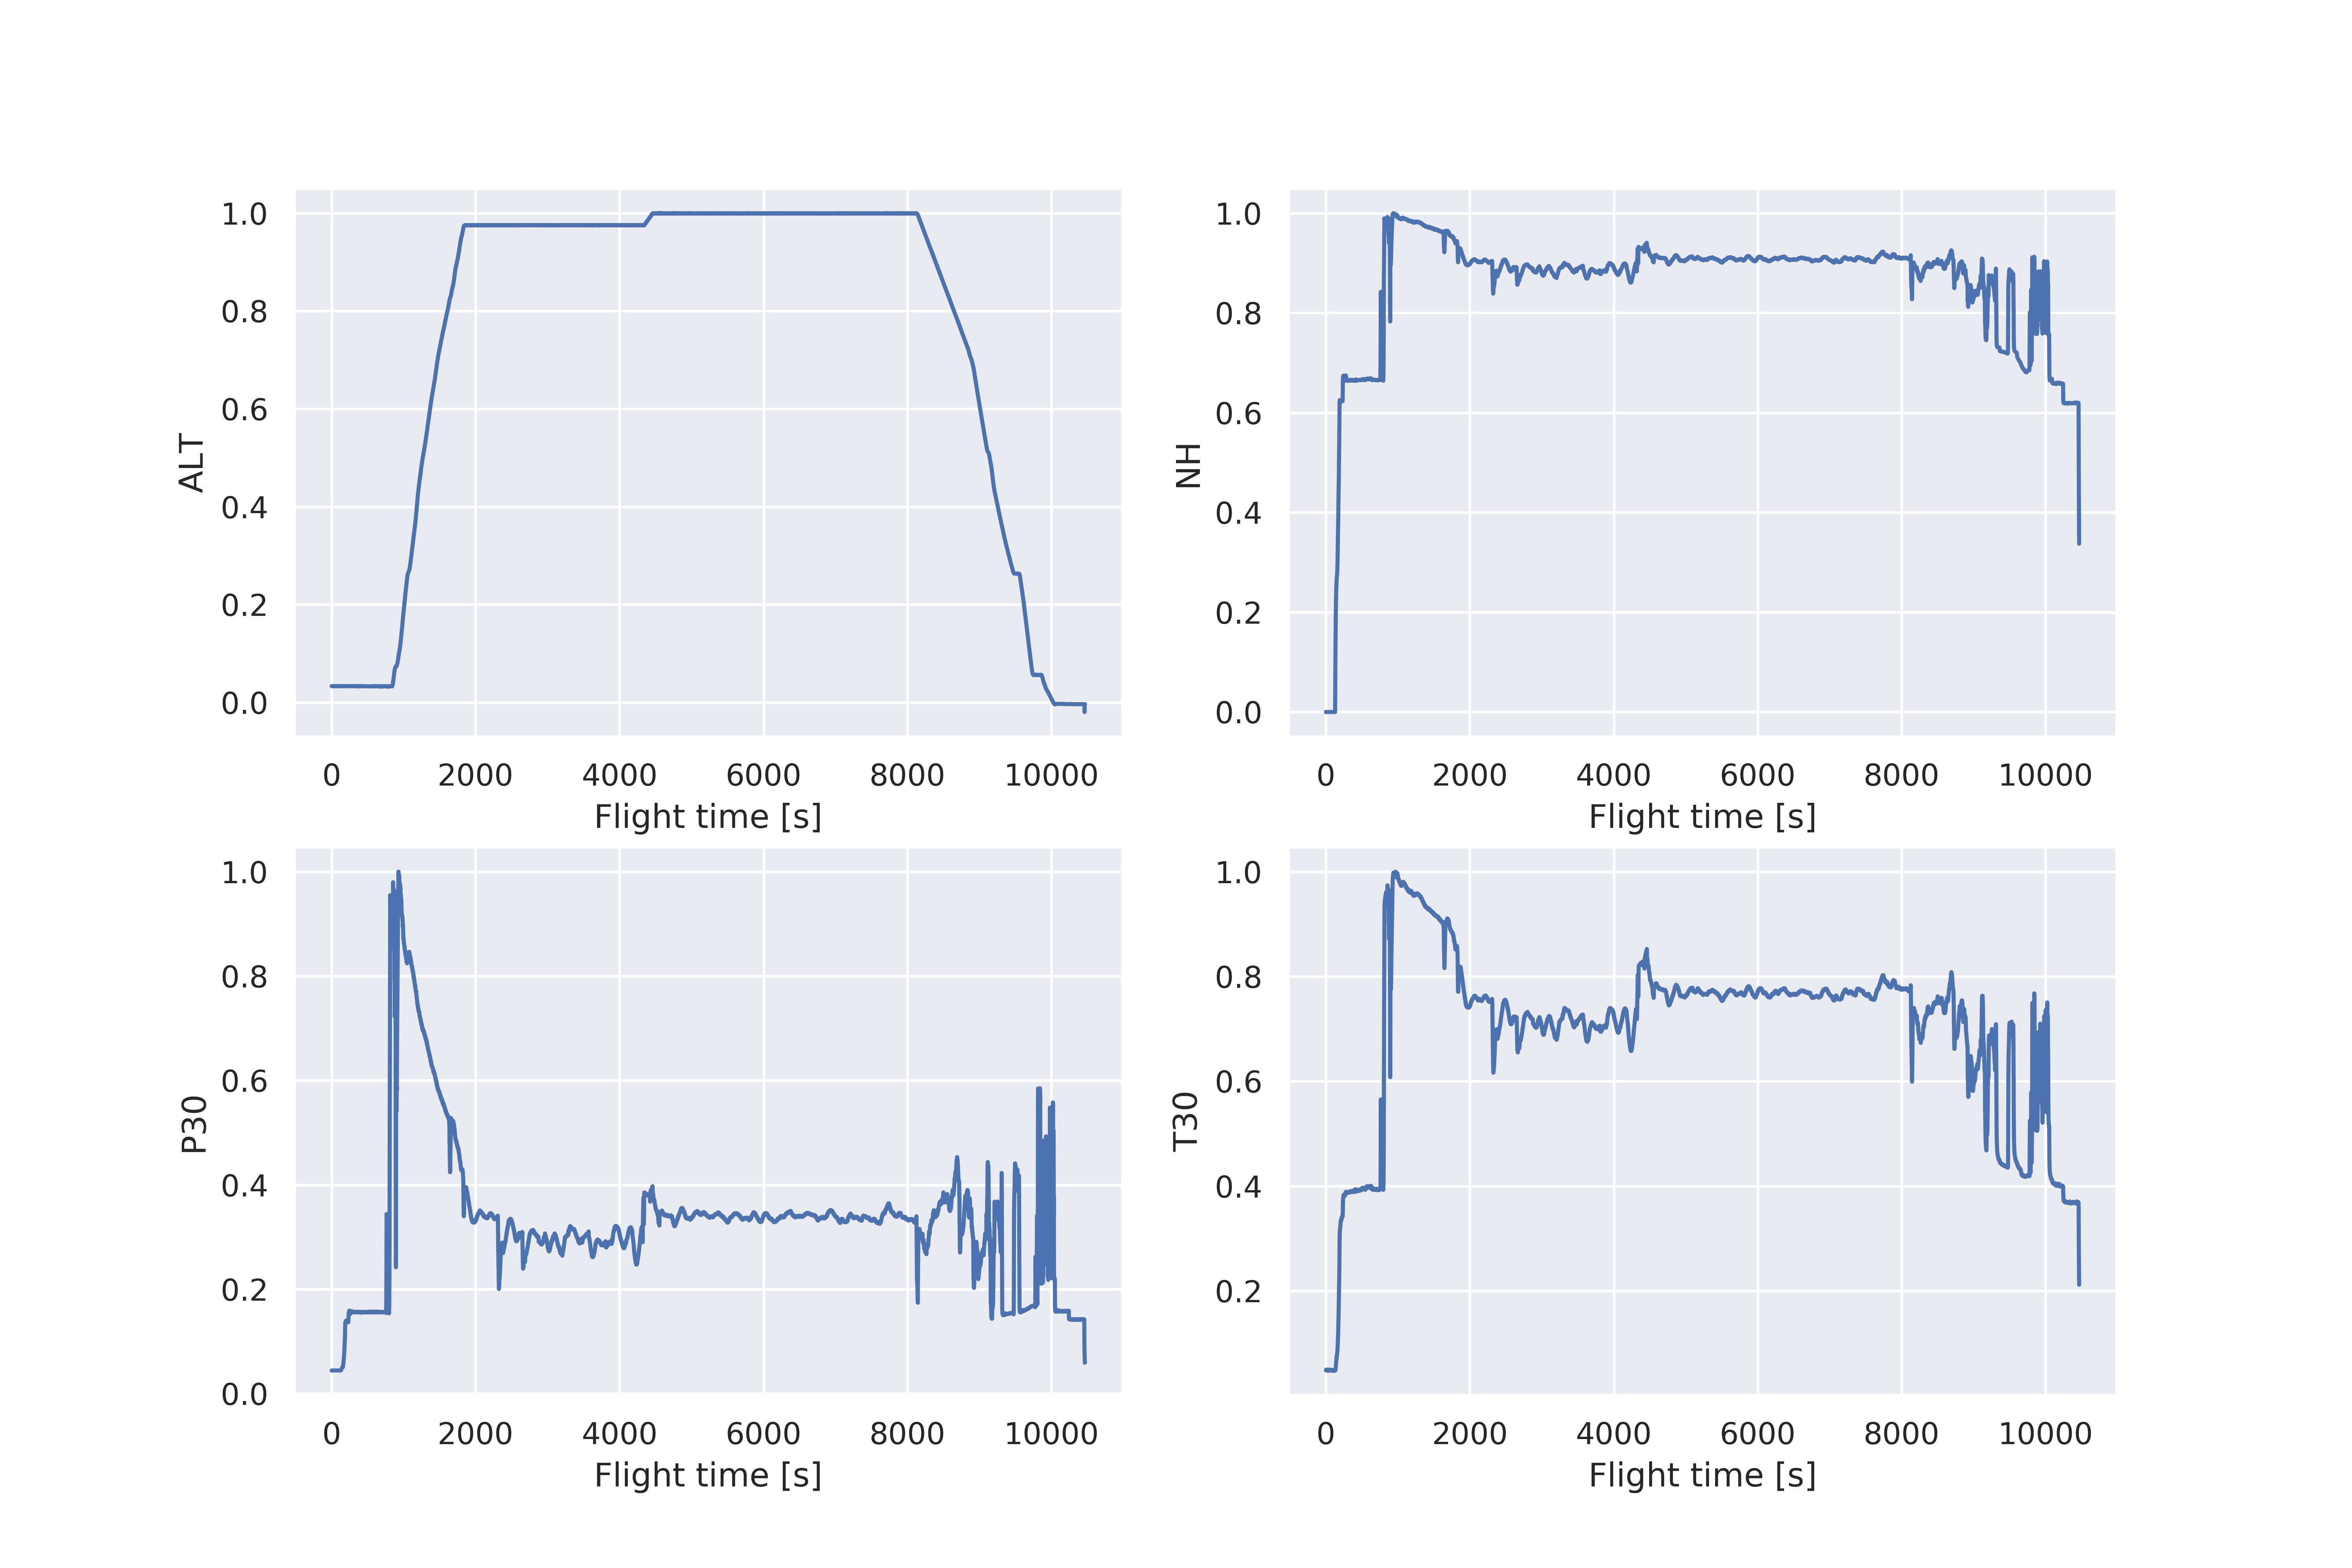
\includegraphics[width=0.9\textwidth]{6008_20150409074414}
    \caption{\label{fig:flt_example} ALT, NH, P30 and T30 of a randomly selected flight. (All parameter values are normalised.)}
\end{figure}

The majority of flights (56.6\%) reached a maximum altitude of \numprint{40000} feet or higher.

\subsection{Flight Phases} \label{sec:phases}
A flight can be split into several phases: preflight, taxi out, take-off, climb, cruise, descent, reverse thrust and taxi in. These phases were extracted using internal Rolls-Royce software \cite[]{konig_br725stats_2015} that combined the flight mode parameter from \ac{ehm} data \cite[]{reischl_br700-725a1-12_2014} and custom conditions for optimisation. The conditions are summarised in table \ref{tab:flight_phases}.

The \ac{fm} often makes use of the parameter \ac{wow}, a boolean parameter with a value of 1 if the aircraft's weight is supported by its wheels, otherwise 0. Other parameters used for determining \ac{fm} include ground speed, intertial vertical speed, wing flap angle and \ac{tra}.

\begin{table}
    \begin{center}
        \caption{\label{tab:flight_phases} Summary of flight phases and conditions at which they begin \cite[]{konig_br725stats_2015}. \ac{fm} conditions in accordance with \citet{reischl_br700-725a1-12_2014}.}
        \begin{tabular}{ l l }
            Phase description & Conditions \\
            \midrule
            Preflight & \ac{fm} \(= 2\) \\
            Taxi out & left or right engine is switched on \\
            Take-off & \ac{fm} \(= 4\) \\
            % & \ac{wow} \(= 1\) \\
            % & \ac{tra} \(> 20^{\circ}\) for both engines \\
            % & ground speed \(> 28\) knots \\
            Climb & \ac{wow} \(= 0\) \\
            & intertial vertical speed \(> 500\) \(\text{ft} / \text{min}\) \\
            & altitude at least \(1500 \) m greater than at take-off \\
            Cruise & \ac{fm} \(= 6\) \\
            & altitude greater than 85\% of maximum altitude \\
            Descent & \ac{fm} \(= 7\) or \ac{fm} \(= 8\) \\
            & \ac{tra} \(< 20^{\circ} \) for both engines \\
            & Time to destination \(< 45\) \(\text{min}\) \\
            Reverse thrust & \ac{fm} \(= 9\) \\
            Taxi in & reverse thrust phase ended
        \end{tabular}
    \end{center}
\end{table}

\subsection{Cycle Counter}
Each flight was processed using SA66 (Section \ref{sa66}) to determine the damage incurred (i.e. the number of cycles consumed).

- One value per feature per flight

- Non-negligible amount of effort required to obtain this data for supervised learning. Big question: Can model scale to smaller data sets?

\subsection{Visualisation}
- Distribution

- Why not centred on 1 cycle if based on "reference" cycle?

- NH-driven, thermally sensitive (F6/F7) - scatter plot F7 divided by F1

\subsection{Downsampling}
- Required for input layer to MLP

- Also better for scalability of models

\subsubsection{(A)PLA}

\subsubsection{APCA}

\subsubsection{Data Loss}
- Average percentage loss caused by downsampling.

- Will it affect model accuracy?

\subsection{Optional: Case Studies}

\subsubsection{6014: Stress Ranges}

\subsubsection{6079: Long Taxi}